\begin{figure}[h!]
    \centering
    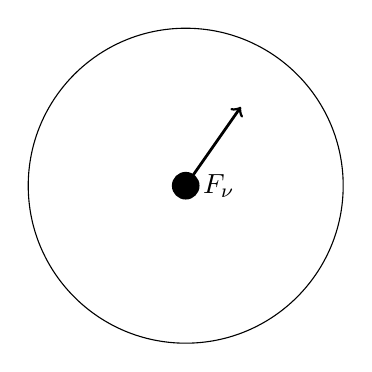
\begin{tikzpicture}
        \fill 
            (0,0) circle[radius=5pt] node[anchor=west]{$\;F_{\nu}$};
        \draw 
            (0,0) circle[radius=2cm];
        \draw 
            [->, black, line width = 1pt] (0,0)--(0.7, 1.0);
    \end{tikzpicture}
    \caption{A hot star surrounded by a cloud of Hydrogen. Note that the cloud doesn't have to be spherical, especially if it posseses an inherent angular momentum, as we'll see in Chapter \ref{ch:vii}.}
    \label{fig:hcloud}
\end{figure}